% Input common header
\documentclass[xcolor=dvipsnames]{beamer}

\usecolortheme[named=Blue]{structure}
\setbeamertemplate{itemize items}[circle]

\usepackage{smartdiagram}


\author{Dr. Paul Larsen}
\date{\today}



\title{Correlation and Causality}
\begin{document}
\maketitle

\begin{frame}
\frametitle{Why causality matters}

   \centering
    \begin{tikzpicture}
 
    \node[inner sep=0pt] (proxy_caption) at (0,0){
        Because correlation is a proxy.
    };

    \node[inner sep=0pt, below=0.5 of proxy_caption] (proxy) at (0,0) {
        \fbox{
            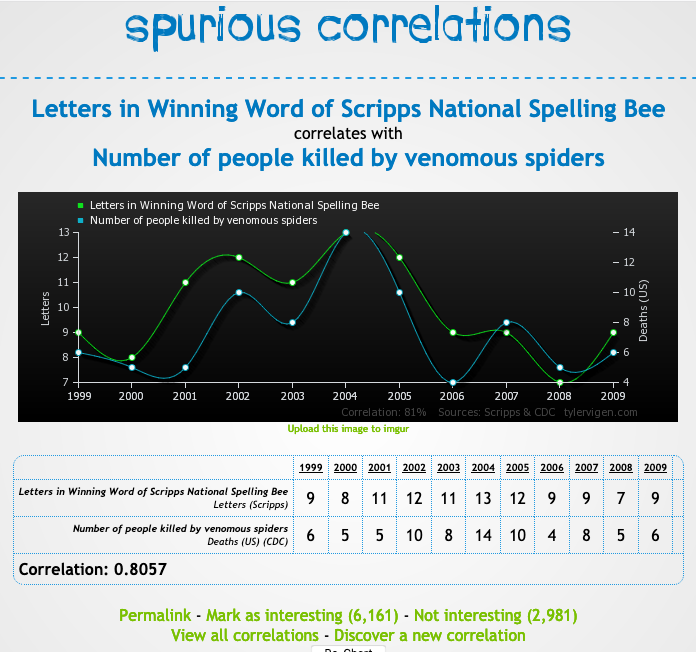
\includegraphics[width=.75\textheight]{graphics/spiders_spelling}
        }
    };
  
\end{tikzpicture}

\cite{spurious-spiders-spelling}
\end{frame}

\begin{frame}
\frametitle{Why causality matters}
\centering
\begin{tikzpicture}

    \node[inner sep=0pt] (med_caption) at (0,0) {
            Because A / B testing is not always possible.
    };
    \node[inner sep=0pt, below=0.5cm of med_caption] (med)  {
        \fbox{
            
\includegraphics[width=.9\textheight]{graphics/mediterranean}
        }
    };
     
\end{tikzpicture}

\cite{estruch2013primary}
\end{frame}


\begin{frame}
    \frametitle{Simpson's paradox: cautionary tales}
    Simpson's paradox: a phenomenon in probability and statistics in which a trend appears disappears or reverses depending on grouping of data. \cite{simpson-wikipedia}, \cite{pearl2016causal} \newline
    
    Example: University of California, Berkeley 1973 admission figures\newline
    
    \begin{figure}[ht]
        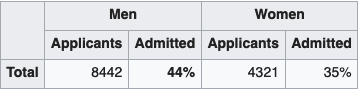
\includegraphics[height=0.15\textheight]{../discrete-geometry/graphics/berkeley}\newline
        \cite{freedman1998statistics}
    \end{figure}
    \begin{figure}[ht]
        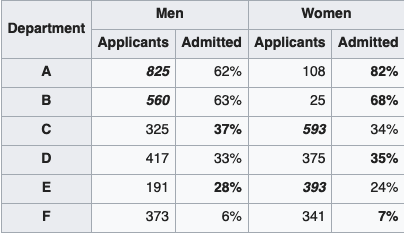
\includegraphics[height=0.3\textheight]{../discrete-geometry/graphics/berkeley_later}\newline
        \cite{Bickel398}
    \end{figure}
    
\end{frame}


\begin{frame}
\frametitle{A brief, biased history of causality}
\begin{itemize}
\item Aristotle, 384 - 322 BC
\item Isaac Newton, 1643 - 1727 AD
\item David Hume, 1711 - 1776 AD
\item Francis Galton, 1822 - 1900 AD, Karl Pearson, 1857 - 1936 AD
\item Judea Pearl, b. 1936 AD
\end{itemize}
\end{frame}


\begin{frame}
\frametitle{Counterfactuals and causality}
Ideal: Intervention + \href{https://en.wikipedia.org/wiki/Multiverse}{Multiverse} $\rightarrow$ Causality\newline

Examples:
\begin{itemize}
\item Medical treatment (e.g. \href{https://en.wikipedia.org/wiki/Simpson\%27s_paradox\#Kidney_stone_treatment}{kidney stone treatment})
\item Social outomes (e.g. \href{https://en.wikipedia.org/wiki/Simpson\%27s_paradox\#UC_Berkeley_gender_bias}{university admissions})
\item Business outcomes (e.g. \href{https://en.wikipedia.org/wiki/Click-through\_rate}{click-through rate}, hit rate)\newline
\end{itemize}

In-practice:
\begin{itemize}
    \item Correlation: approximate multiverse by comparing intervention at $t$ to result at $t-1$
    \item Random population: approximate multiverse by splitting sample well
    \item A / B testing: random populations A / B + intervention in one
\end{itemize}
\end{frame}




\begin{frame}
\frametitle{Counterfactual example: hit rate for insurance}
Variables:
\begin{itemize}
\item product\_type: Client line of business
\item days: Number of days to generate quote
\item rating: Binary indication of client risk
\item hit: Binary, 1 for success (binding the quote), 0 for failure\newline
\end{itemize}

Fake data:\newline\newline
\begin{tabular}{lrrr}
\toprule
product\_type &  days &  rating &  hit \\
\midrule
    property &     3 &       1 &    0 \\
   liability &     1 &       0 &    0 \\
   financial &     0 &       1 &    0 \\
   liability &     3 &       0 &    0 \\
   liability &     0 &       0 &    1 \\
\bottomrule
\end{tabular}
\newline
\end{frame}


\begin{frame}
    \frametitle{Counterfactual example: hit rate for insurance}
    Variables:
    \begin{itemize}
    \item product\_type: Client line of business
    \item days: Number of days to generate quote
    \item rating: Binary indication of client risk
    \item hit: Binary, 1 for success (binding the quote), 0 for failure\newline
    \end{itemize}
    
    \begin{figure}[ht]
    \includegraphics[height=0.6\textheight]{graphics/hit}
    \end{figure}
\end{frame}



\begin{frame}
\frametitle{Non-counterfactual approach: condition and query}

Goal: estimate effect of $\textrm{days}$ on $\textrm{hit}$.\newline

Calculate
\begin{itemize}
\item $P(\textrm{hit}=1 | \textrm{days} = 0) - P(\textrm{hit}=1 | \textrm{days} = 1)$,
\item $P(\textrm{hit}=1 | \textrm{days} = 1) - P(\textrm{hit}=1 | \textrm{days} = 2)$,
\item $\ldots$ \newline
\end{itemize}

From exercise Jupyter notebook:\newline
\begin{tabular}{lr}
\toprule
{} &       hit \\
days &           \\
\midrule
0    &  0.539135 \\
1    &  0.440035 \\
2    &  0.326531 \\
3    &  0.168289 \\
\bottomrule
\end{tabular}

\end{frame}


\begin{frame}
    \frametitle{The Structural Causal Model}
    The definitions in following slides are from \cite{pearl2007mathematics}, \cite{pearl2016causal}.
\begin{definition}
    A \emph{structural causal model} $M$ consists of two sets of variables $U, V$ and a set of functions $F$, where 
    
    \begin{itemize}
        \item $U$ are considered \emph{exogenous}, or background variables, 
        \item $V$ are the \emph{causal} variables, i.e. that can be manipulated, and
        \item $F$ are the functions that represent the process of assigning values to elements of $V$ based on other values in $U, V$, e.g. $v_i = f(u, v)$.
    \end{itemize}

    We denote by $G$ the graph induced on $U, V$ by the functions $F$, and call it the \emph{causal graph} of $(U, V, F)$.\newline
\end{definition}

Hit rate example: $U = \{\textrm{product\_type}, \textrm{rating}\}$, $V= \{\textrm{days}, \textrm{hit}\}$, $F\leftrightarrow$ sample from conditional probabilty tables in directed graphical model.
\end{frame}


\begin{frame}
    \frametitle{Formalizing interventions: the intuition of ``do"}
    For business application, quantity of interest is not $P(\textrm{hit}=1 | \textrm{days}=d)$, but intervention $$P(\textrm{hit}=1 | \jpdo(\textrm{days}=d))$$.\newline
    \begin{figure}[ht]
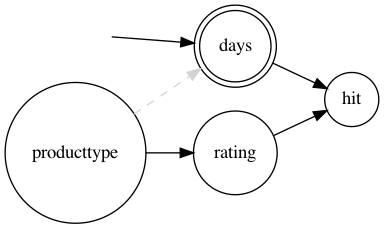
\includegraphics[height=0.4\textwidth]{graphics/do_days}
    \end{figure}
\end{frame}


\begin{frame}
\frametitle{Formalizing interventions: the intuition of ``do"}
    For business application, quantity of interest is effect of intervention / counterfactual %$P(\textrm{hit}=1 | \textrm{days}=d)$, but intervention $$P(\textrm{hit}=1 | \jpdo(\textrm{days}=d))$$.\newline
\begin{columns}[T] % align columns
    \begin{column}{.48\textwidth}
    Not $P(\textrm{hit}=1 | \textrm{days}=d)$\newline
    \begin{figure}[ht]
        $G = $ 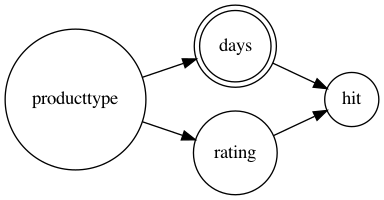
\includegraphics[height=0.55\textwidth]{graphics/given_days}
    \end{figure}
    \end{column}%
%    \hfill%
    \begin{column}{.48\textwidth}
        but $P(\textrm{hit}=1 | \jpdo(\textrm{days}=d))$\newline
               \begin{figure}[ht]
             $G' = G_{\underline{\textrm{days}}} =$
             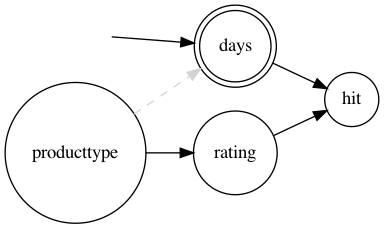
\includegraphics[height=0.55\textwidth]{graphics/do_days}
        \end{figure}
         \end{column}%
    \end{columns}
\end{frame}


\begin{frame}
\frametitle{Formalizing interventions: the intuition of ``do"}
	First, find quantities unchanged between $G$ and $G' = G_{\underline{\textrm{days}}}$
         \begin{figure}[ht]
             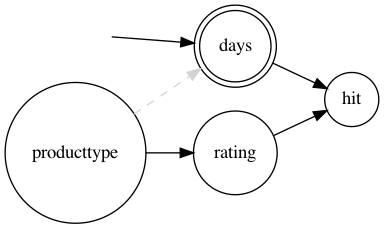
\includegraphics[height=0.5\textheight]{graphics/do_days}
        \end{figure}
        \vspace{-0.5cm}
        \begin{align}
        P_{G'}( & \textrm{product\_type} = p, \textrm{rating} = r) \nonumber \\
        & = P_G( \textrm{product\_type} = p, \textrm{rating} = r) \\
        P_{G'}(&\textrm{hit}=1 | \textrm{product\_type} = p, \textrm{rating} = r) \nonumber  \\
        & = P_G(\textrm{hit}=1 | \textrm{product\_type} = p, \textrm{rating} = r)
        \end{align}
\end{frame}


\begin{frame}
\frametitle{Formalizing interventions: the intuition of ``do"}
	\vspace{-1.5cm}
	\begin{figure}[ht]
	\hspace{8cm}
             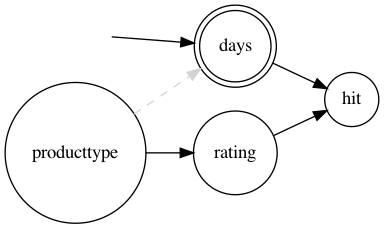
\includegraphics[height=0.45\textheight]{graphics/do_days}
        \end{figure}
        \vspace{-2.5cm}
        \begin{align*}
         P(&\textrm{hit}=1 | \jpdo(\textrm{days})=d) \\
         & = P_{G'}(\textrm{hit}=1 | \textrm{days}=d) \textrm{, by definition} \\
        & = \sum_{p, r} P_{G'}(\textrm{hit}=1 | \textrm{days}=d, \textrm{product\_type} = p, \textrm{rating} = r) \\
        & \qquad  \qquad P_{G'}(\textrm{product\_type} = p, \textrm{rating} = r | \textrm{days}=d)\textrm{, by total probability} \\
        & = \sum_{p, r} P_{G'}(\textrm{hit}=1 | \textrm{days}=d, \textrm{product\_type} = p, \textrm{rating} = r) \\
        & \qquad  \qquad P_{G'}(\textrm{product\_type} = p, \textrm{rating} = r), \textrm{ by substitution} \\
        & =  \sum_{p, r} P_{G}(\textrm{hit}=1 | \textrm{days}=d, \textrm{product\_type} = p, \textrm{rating} = r) \\
        & \qquad  \qquad P_{G}(\textrm{product\_type} = p, \textrm{rating} = r), \textrm{ our \emph{adjustment} formula} 
        \end{align*}
        References: \cite{pearl2016causal}, \cite{chmp}
\end{frame}


\begin{frame}
\frametitle{Causal hit rate}
\begin{columns}[T] % align columns
    \begin{column}{.48\textwidth}
    $P(\textrm{hit}=1 | \textrm{days}=d)$\newline
    
    \begin{tabular}{lr}
\toprule
{} &       hit \\
days &           \\
\midrule
0    &  0.539135 \\
1    &  0.440035 \\
2    &  0.326531 \\
3    &  0.168289 \\
\bottomrule
\end{tabular}

    \end{column}%
%    \hfill%
    \begin{column}{.48\textwidth}
        $P(\textrm{hit}=1 | \jpdo(\textrm{days}=d))$\newline
        
          \begin{tabular}{rr}
\toprule
 days &      prob \\
\midrule
    0 &  0.555426 \\
    1 &  0.409581 \\
    2 &  0.274834 \\
    3 &  0.196311 \\
\bottomrule
\end{tabular}


         \end{column}%
    \end{columns}

\end{frame}

\begin{frame}
\frametitle{Judea Pearl's Rules of Causality}

Let $X$, $Y$ , $Z$ and $W$ be arbitrary disjoint sets of nodes in a DAG $G$. Let $G_\underline{X}$ be the graph obtained by removing all arrows pointing into (nodes of) $X$. 
Denote by $G_{\overline{X}}$ the graph obtained by removing all arrows pointing out of $X$. If, e.g. we remove arrows pointing out of $X$ and into $Z$, we the resulting graph is denoted by $G_{\underline{X} \overline{Z}}$

Rule 1: Insertion / deletion of observations
\begin{equation*}
P(y | \jpdo(x), z, w) = P(y | \jpdo(x), w) \textrm{ if } (Y \ci Z | X, W)_{G_{\overline{X}}}
\end{equation*}

Rule 2: Action / observation exchange
\begin{equation*}
P(y | \jpdo(x), \jpdo(z), w) = P(y | \jpdo(x), z, w) \textrm{ if } (Y \ci Z | X, W)_{G_{\overline{X} \underline{Z}}}
\end{equation*}

Rule 3: Insertion / deletion of actions
\begin{equation*}
P(y | \jpdo(x), \jpdo(z), w) = P(y | \jpdo(x), w) \textrm{ if } (Y \ci Z | X, W)_{G_{\overline{X} \overline{Z(W)}}},
\end{equation*}

where $Z(W)$ is the set of $Z$-nodes that are not ancestors of any $W$-node in $G_\underline{X}$.

\end{frame}


\begin{frame}
\frametitle{Special cases of the causal rules}

By judicious setting of sets of nodes to be empty, we obtain some useful corollaries of the causal rules.
\newline

Rule 1': Insertion / deletion of observations, with $W = \emptyset$
\begin{equation*}
    P(y | \jpdo(x), z) = P(y | \jpdo(x)) \textrm{ if } (Y \ci Z | X)_{G_{\overline{X}}}
\end{equation*}

Rule 2': Action / observation exchange, with $X = \emptyset$
\begin{equation*}
P(y | \jpdo(z), w) = P(y | z, w) \textrm{ if } (Y \ci Z | W)_{G_{ \underline{Z}}}
\end{equation*}

Rule 3': Insertion / deletion of actions, with $X, W = \emptyset$
\begin{equation*}
P(y | \jpdo(z)) = P(y) \textrm{ if } (Y \ci Z )_{G_{\overline{Z}}}
\end{equation*}

\onslide<2->\textcolor{blue}{$\implies$ d-separation + causal rules = \emph{adjustment formulas}: $\jpdo$ queries as normal queries.}
\end{frame}


\begin{frame}[allowframebreaks]
    \frametitle{References}
    \setbeamertemplate{bibliography item}[text]
    \bibliographystyle{amsalpha}
    \bibliography{../references.bib}
\end{frame}

\end{document}